\documentclass[main.tex]{subfiles}
\begin{document}



\chapter{Background}

% TODO
% - terminologie compilation toolchain
% - infer block ram during compilation

\section{Field-programmable gate arrays}
Field-programmable gate arrays (FPGA) are a class of integrated circuits (IC) which' behaviour is reconfigurable, as opposed to application specific integrated circuits (ASIC). In general, FPGAs consist of blocks of configurable logic which are interconnected through a configurable network. While some of a FPGA's physical pins are reserved, a majority of a FPGA's pins are generally available to user I/O and are exposed internally through I/O blocks (IOB). Manufacturers combine configurable logic blocks (CLB) with additional static functionality ranging from primitives such as memory elements to complex functionality such as embedded microprocessors. The included static functionality differs per FPGA model and manufacturer and many different variations currently exist, targeted at various applications.

\begin{figure}[h]
    \centering
    \caption{A basic view of a FPGA configurable logic block, derived from \cite{Kallstrom2010fpga}. The block supports synchronous operation through the integrated flip-flop (FF).}
    \label{fig:fpga-clb}
    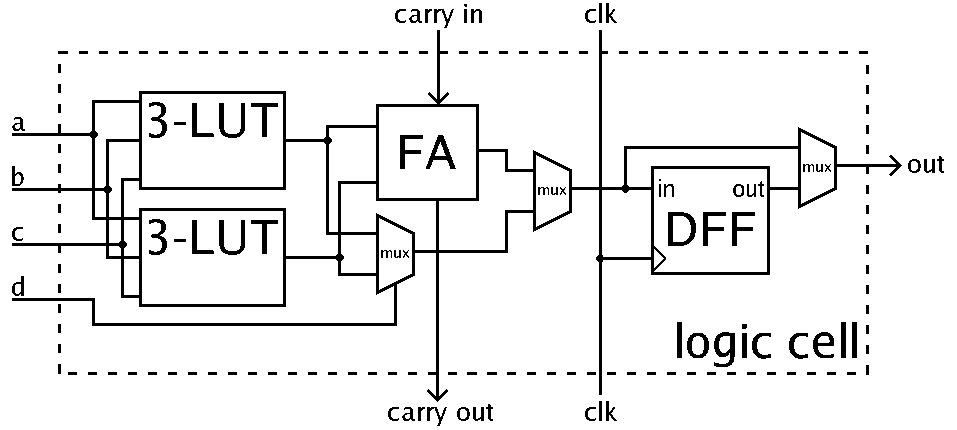
\includegraphics[width=0.7\textwidth]{img/fpga-clb}
\end{figure}

In its most primitive form, a FPGA CLB can be described as a lookup table (LUT) whose output is optionally buffered by a flip-flop, as displayed in figure \ref{fig:fpga-clb}. The LUT can be configured to capture combinational logic and the flip-flip is added in order to support synchronous operation such that the CLB can be configured to capture synchronous sequential logic. This simplistic view does not represent the CLBs as used in the designs of FPGA manufacturers, however. As can be seen in \cite{ug474}, a Xilinx 7 series FPGA's CLBs are significantly more complex. Manufacturers include more functionality in CLB designs such that these can be used more efficiently to serve as memory elements or perform arithmetic operations, for example.

\begin{figure}[h]
    \centering
    \caption{A basic view of a FPGA's architecture, derived from \cite[Fig.2]{szedoAboutFpgas}. CLBs are aligned in a symmetrical array. The gray boxes and interconnecting lines represent the FPGA's configurable interconnects. The blue lines represent the FPGA's clock delivery network. I/O blocks (IOB) serve as entry points to FPGA pins.}
    \label{fig:fpga-architecture}
    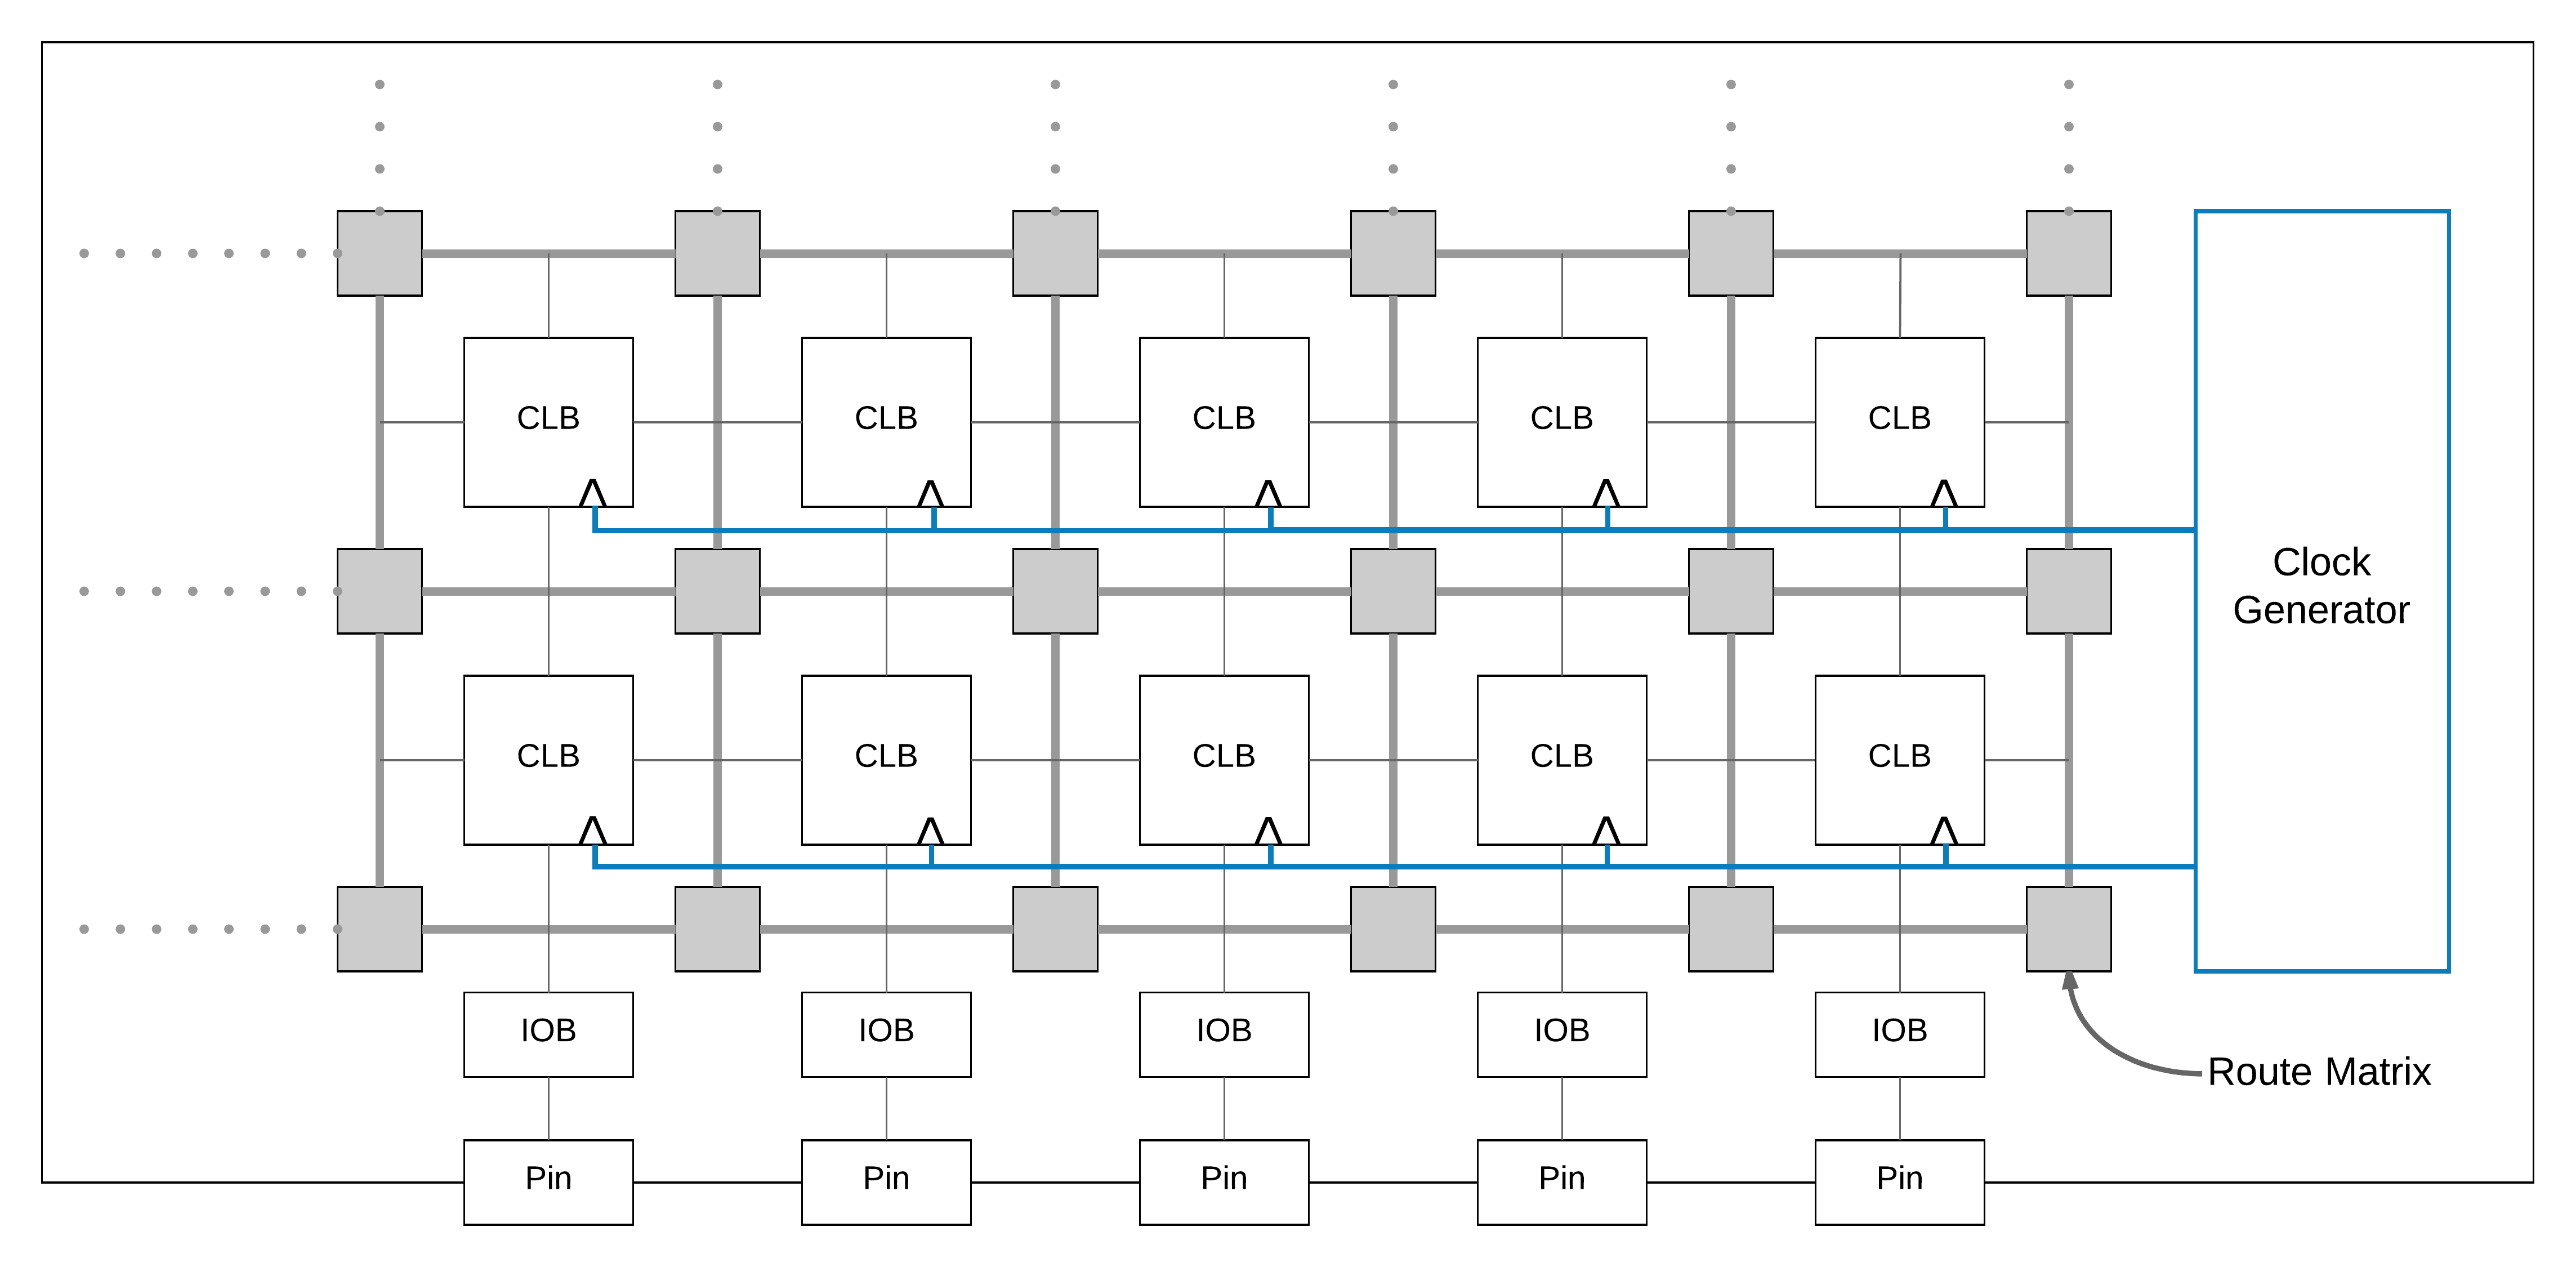
\includegraphics[width=\textwidth]{img/fpga-architecture}
\end{figure}

In order to combine multiple blocks of logic, CLB inputs and outputs need to be interconnected. FPGA manufacturers adopt different topologies in designing their CLB interconnect networks. Although different in structure, these networks share the capability of being reconfigurable such that routes may be defined between different blocks' input and output ports. Figure \ref{fig:fpga-architecture} displays a FPGA architecture in which the CLBs and their interconnects are aligned in a symmetrical array structure. As described in \cite[Fig.2]{szedoAboutFpgas}, other topologies can be adopted as well. Row-based and hierarchical structures for example, are other types of structures adopted by manufacturers in their FPGA designs.  

\section{FPGA Clocking Resources}
\label{section-fpga-clocking-resources}
In order for CLBs to be configured as elements of synchronous sequential logic, the CLB requires a clock input signal. Distributing this clock signal through the configurable CLB interconnect network however, causes an unpredictable amount of clock skew accross different CLB clock inputs. In order to overcome this unpredictability, FPGAs are generally equipped with a dedicated clock delivery network. The blue lines in figure \ref{fig:fpga-architecture} represent such a clock delivery network. Manufacturers adopt different design strategies in order to minimize clock skew accross their FPGAs. As can be seen in \cite{cv5v2} for example, the Altera Cyclone V class of FPGAs feature a clock delivery network that is defined hierarchically. 

Additional to dedicated logic for clock delivery, current FPGAs generally offer some configurable functionality for synthesis, selection and manipulation of clock signals. Several independent clock signals of different frequencies can be derived from a base signal through multiplication and routed to different sections on the FPGA. This base signal is usually provided by an external clock generating device. Besides clock synthesis and routing, FPGAs generally feature buffers that allows for 'gating' of clock signals through which a specific clock signal may be (regionally) disabled through user-defined logic. The technique of clock gating is generally used to disable state transitions in a particular section of an IC in order reduce power consumption. In this thesis however, this technique will be utilized to generate clock pulses with irregular intervals.

% Figure \ref{fig:fpgastructure} gives a structural overview of a FPGA as manufactured by Xilinx. It shows a number of CLBs, interconnected with I/O blocks (IOB) that connect IC package pins and block rams (BRAM) which serve as static blocks of memory. The digital clock manager (DCM) is responsible for the distribution of clock signals to every of the FPGA's blocks. A CLB's contained logic is described through an internal lookup table in which 

% \begin{figure}
% \centering
% 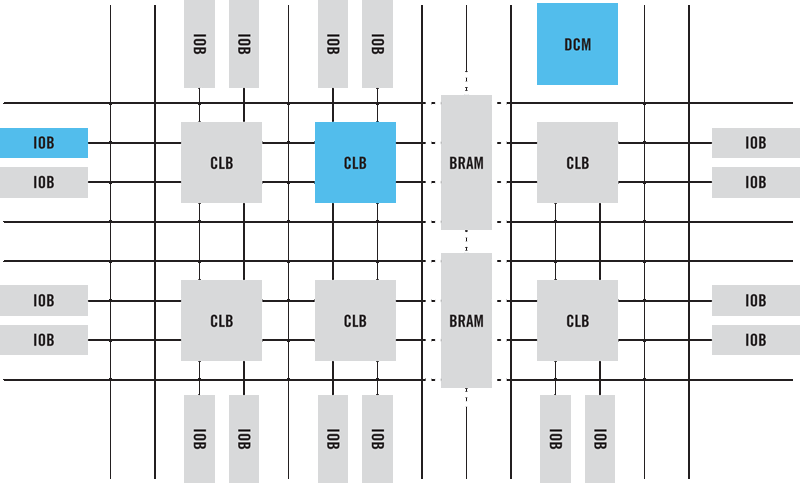
\includegraphics[width=.7\textwidth]{img/fpga-block-structure}
% \caption{Structural FPGA overview}
% \label{fig:fpgastructure}
% \end{figure}

% \begin{figure}
% \centering
% 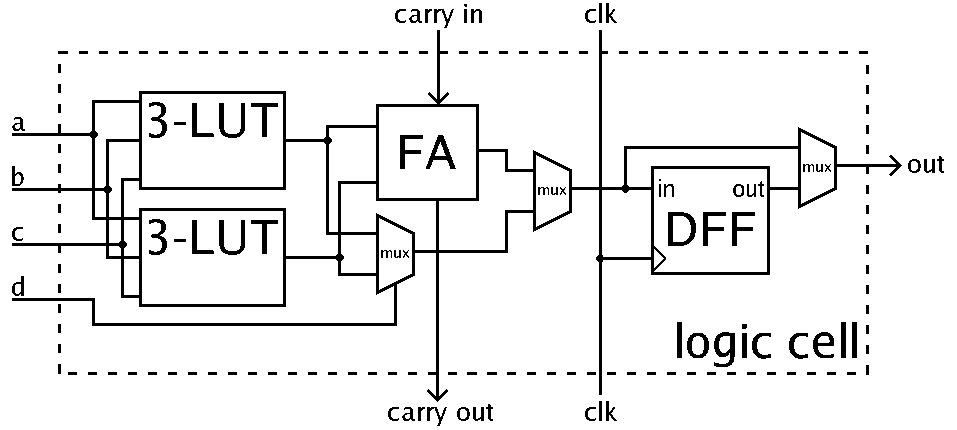
\includegraphics[width=.7\textwidth]{img/fpga-clb}
% \caption{FPGA CLB example overview}
% \label{fig:my_label}
% \end{figure}



\section{FPGA Development Process}
% The FPGA development process is targeted at the creation of a new FPGA configuration. 

Developers generally define their designs' logic on a register-transfer level (RTL) through some hardware definition language (HDL), such as Verilog or VHDL. In order for these designs to be translated into a FPGA configuration, these designs are first processed by a logic synthesizer. The goal of the logic synthesis process is to translate the hierarchical RTL logic representation into a 'flat' netlist representation which is composed of elements that correspond with FPGA primitives.

In order to translate the primitive netlist representation into a FPGA configuration, the design is processed in the implementation process. During this process, the netlist primitives are first mapped onto FPGA elements, but not assigned to a location yet. Users are generally capable of controlling the implementation process through specification of constraints, such as specific timing requirements. After succesfully mapping, the exact location has to be determined such that routes between the elements' inputs and outputs can be established while satisfying the user-defined constraints. This process of finding a suitable combination of locations and routes is generally the most time-consuming of all operations. Once successful, the configuration is written to a FPGA-specific binary format such that is suitable for programming the FPGA. This type of file is commonly referred to as a bitstream file. 

Although some third-party synthesis tools are available, the implementation process is generally facilitated by proprietary tools supplied by the FPGA's manufacturer, since many of the implementation process' details are based on proprietary information. Manufacturers generally bundle their development tools into a software development kit (SDK) which includes an integrated development environement (IDE) for interacion with these tools through a graphical interface. Even though the graphical interface is often a developer's primary means of interaction, scripted operation of these development tools is possible as well. The development tools developed as part of this thesis focus on scripted operation of the FPGA development process.


\section{FPGA Development Boards}
FPGAs are used in a wide range of products in which they are statically configured to perform specific tasks. There is a class of products however, that preserves the FPGA's reconfigurable behaviour and exposes this functionality directly to its end users. These products are typically used for development of new logic configurations and essentially serve as a tool during the development process. A FPGA development board generally includes a number of I/O devices for human interaction, sensory input or machine-to-machine communication. These devices range from simple LEDs and switches to external ICs with advanced functionalities. Furthermore, FPGA development board are generally equipped with pins for general purpose I/O with external devices. FPGA development boards range from boards with simple, general-purpose peripheral devices from boards with high-end components targeted at specific goals, such as digital signal processing.

One class of I/O devices that will prove of particular relevance to this thesis are the devices used for board-to-PC communication. FPGA development boards generally include some means to support the establishment of a serial point-to-point communication channel. The board generally features the electronics that allow physical compatibility with the communication medium, while the remaining higher-level logic such as an UART, is implemented in the user-defined logic contained within the FPGA. Traditionally, board-to-PC communication was often established through a RS-232 connection, but current development boards generally allow for establishing a virtual point-to-point communication channel over USB through a USB-UART bridge. Additional to a USB interface, modern boards are often equipped with an Ethernet interface as well, allowing for networked communication.  

\section{FPGA Configuration}

FPGAs generally reserve a number of pins for the purpose of configuration. The terms programming and configuration may be used interchangeably. Current FPGAs generally make use of the IEEE 1532 standard for in-system programming, which extends the IEEE 1149.1 'JTAG' boundary scan protocol. Although some boards require third-party programming hardware, current FPGA development boards often include some form of programming circuitry that allows for reconfiguration of the FPGA through the user's PC.

Although the FPGA's programming interface may often be considered universal, the PC software required for programming is generally targeted at specific proramming hardware. However, FPGA manufacturers often bundle programming drivers for their and their third party partners' boards in their SDKs. Additionally, FPGA manufacturers such as Xilinx and Altera provide smaller 'lab' editions of their SDKs that only include the tools and drivers required for configuration. Through these programming tools, the user is capable of uploading a bitstream file that was previously created during the development process.



\end{document}